\documentclass{article}

% basic latex template Seminararbeit ML in Robotics
% adapted from overleaf example

% Language setting
% Replace `english' with e.g. `spanish' to change the document language
\usepackage[english]{babel}

% Set page size and margins
% Replace `letterpaper' with `a4paper' for UK/EU standard size
\usepackage[a4paper,top=2cm,bottom=2cm,left=3cm,right=3cm,marginparwidth=1.75cm]{geometry}

% Useful packages
\usepackage{amsmath}
\usepackage{graphicx}
\usepackage[colorlinks=true, allcolors=blue]{hyperref}

\usepackage{url}

\title{Robot Skill Learning without a Cost Function: Optimization of Dynamic Movement Primitives via Naive User Feedback"}
\author{Simon Maximilan Friedo, Marvey Bano, Sedra Abou Ghaloun\\\\Seminar Machine Learning in Robotics - WiSe2023/24\\Humboldt-Universit\"at zu Berlin}

\begin{document}
    \maketitle

    \begin{abstract}
        Teaching a robot a skill without the need of a complex cost function would enable naive users to teach their robots
        new tasks by themselves.
        This seminar paper aims to replicate the approach that Vollmer et al. represented in their paper "A User Study on Robot Skill
        Learning Without a Cost Function: Optimization of Dynamic Movement Primitives via Naive User Feedback" ~\cite{vollmer2018}.
        To replicate the approach we simulated pepper using qibullet and used the dmpbbo package ~\cite{stulp2019dmpbbo} to learn
        a movement using naive user feedback.
    \end{abstract}


    \section{Introduction}
    Robots are becoming increasingly integrated into our daily lives, necessitating learning mechanisms that are accessible to all users.
    While Programming by Demonstration (PbD) allows users to demonstrate tasks to robots, some tasks require precise movements
    that are challenging to convey through demonstration alone.
    Consequently, self-improvement from imperfect demonstrations is often more practical.
    However, existing research on robot learning tends to prioritize task performance optimization over user usability, with
    PbD studies primarily conducted in controlled laboratory settings and rarely involving non-expert users.
    \newline A User Study on Robot Skill Learning Without a Cost Function: Optimization of Dynamic Movement Primitives via Naive User
    Feedback~\cite{vollmer2018} aims to investigate the feasibility of employing state-of-the-art optimization systems in a
    user-centric context, focusing on intuitive usability and applicability outside the laboratory.
    Specifically, exploring robot learning of complex movement skills with human teachers, utilizing Dynamic Movement Primitives
    (DMPs) as a widely adopted method from the PbD literature.
    \newline While human-provided feedback is often considered noisy and unreliable, Vollmer et al.~deliberately opt to use an
    unaltered optimization system without specific adaptations for human-provided signals with the objective is to establish
    a baseline performance of a PbD setup trained solely on human feedback.
    The only modification introduced is replacing sensory-based cost evaluation with an intuitive graphical user interface,
    allowing users to provide discrete feedback after each movement execution.
    \newline In this seminar paper we aim to implement the approach outlined in the paper.
    Our strategy involves integrating a state-of-the-art optimization system by using the dmpbbo package~\cite{stulp2019dmpbbo}.
    with a simple terminal based interface that enables non-expert users to provide feedback easily.
    In the absence of a physical Pepper Robot we will utilize QiBullet~\cite{QiBullet} Simulation.
    This interface will allow users to offer discrete-valued feedback to the simulated robot after each movement execution
    facilitating a more interactive and collaborative learning process.
    We will utilize Dynamic Movement Primitives (DMPs) as the underlying method for robot learning in combination with
    black box optimization as described in~\cite{stulp2019dmpbbo}.
    \section{Related work/Literature}

    We only used the paper A User Study on Robot Skill Learning Without a Cost Function: Optimization of Dynamic
    Movement Primitives via Naive User Feedback~\cite{vollmer2018} and the git from the dmpbbo package~\cite{stulp2019dmpbbo}.
    During our research we also saw multiple project utilizing the dmpbbo package to teach a robot different kind of tasks.
    Sadly those project did lack source code and are therefore not used for this seminar paper.
    The Paper by Vollmer et al.~\cite{vollmer2018} also lacked source code which lead to us using mostly the examples
    from the dmpbbo package~\cite{stulp2019dmpbbo} as well as the description of the model form the paper to
    approximate the model for learning trajectories.
    We had to make multiple assumptions about details of the model that the paper omitted.


    \section{Own approach}
    Our approach was to reimplement the basic functionality presented in the study and substitute a real pepper robot with a
    simulation.
    Our own approach consisted of generating an initial trajectory using an array of joint configurations for five joints of
    the right arm and utilizing the build in from\_polynomial method of the Trajectory Class from the dmpbbo
    package~\cite{stulp2019dmpbbo}.
    We then simulated the trials using Qibullet \cite{QiBullet} and provided naiv feedback with a number from 1 (not good at
    all) up to 5 (very good) using the terminal.
    The inverted feedback was then used as feedback for the learning algorithm.
    The learning algorithm consists of a black box optimization of dynamical movement primitives utilizing function approximates.

    \subsection{Simulation}
    In the absence of a physical Pepper Robot, the challenge of simulating its movements for interactive machine learning
    was effectively addressed through the utilisation of QI Bullet.
    QiBullet is the tool which allows the simulation of the robot in a virtual environment~\cite{QiBullet}.
    This trial aimed to replicate the dynamics outlined in the project's instructions, facilitating machine learning via
    user feedback.
    \newline The simulation process started with the specification of joint movements within Pepper's arm.
    Notably, RShoulderPitch, RElbowYaw, and RElbowRoll were identified as pivotal joints for the desired movements.
    By assigning different values to these joints, the simulation aimed to emulate Pepper's gestures accurately.
    \newline To initiate movement, initial joint configurations were manually inputted, to state the starting positions of each joint
    and their respective speeds.
    This input facilitated the simulation of sequential movements, enabling the visualisation of Pepper's actions within the
    QI Bullet environment on the computer screen.
    While the replication of the game described in the original paper was impeded by the inability to spawn objects, the
    focus remained on achieving realistic movement dynamics.
    Despite this limitation, the simulation strived to capture the essence of Pepper's gestures, thereby enabling an
    immersive user experience.
    Central to the interactive machine learning aspect was the incorporation of user feedback.
    Users were prompted to evaluate the simulated movements based on their perceived accuracy and efficacy.
    Subsequently, new values were assigned to the joint movements, thereby refining Pepper's actions in response to user input.
    The feedback loop was integral to the iterative improvement of Pepper's movements.
    Users could input values ranging from 1 (indicating poor performance) to 5 (denoting good execution) via the terminal interface.
    These evaluations informed subsequent adjustments, empowering the simulated robot to progressively enhance its movement repertoire.
    \newline The movement to be replicated in the simulation was a precise arm motion executed by the Pepper Robot to maneuver a small ball into a cup. In the game scenario, the ball was tethered to the cup with a string, adding an additional layer of complexity to the task.
    The arm movement required coordination of multiple joints, specifically RShoulderPitch, RElbowYaw, and RElbowRoll. These joints would work together to position Pepper's arm in a manner conducive to guiding the ball towards the cup.

    \begin{itemize}
        \item Initial Movement Attempt: Pepper's arm would be positioned to hold the cup as described previously. The swinging ball, although unseen by Pepper, would be simulated to swing within a defined range.
        \item User Feedback Prompt: After each movement attempt, users would be prompted to provide feedback on the accuracy of Pepper's positioning and timing. This feedback would serve as the primary indicator of whether the movement was successful in catching the swinging ball.
        \item Evaluation of User Feedback: The user feedback, provided through the terminal interface as described earlier, would be evaluated to determine the effectiveness of Pepper's movement. Users might rate the attempt based on factors such as the alignment of the cup with the swinging ball, the timing of the catch, and the stability of the cup during the catch.
        \item Adjustment of Movement Parameters: Based on the user feedback, adjustments would be made to Pepper's arm movement parameters, such as joint angles and speed, for subsequent attempts. The goal would be to iteratively refine Pepper's movements to better align with user expectations.
        \item Iterative Improvement: Through successive iterations of movement attempts and user feedback, Pepper's simulated movements would gradually improve in accuracy and effectiveness. Users would continue to provide feedback, guiding the simulation towards achieving the desired level of performance in catching the swinging ball.
    \end{itemize}
    
    In this adaptation, the user's subjective evaluation becomes the primary mechanism for assessing the correctness of Pepper's movements. By incorporating user feedback into the iterative learning process, the simulated robot can refine its actions to better align with user expectations, despite the absence of direct visual observation.
    In essence, the simulation achieved a commendable emulation of Pepper's movements through the adept utilisation of QI Bullet. By integrating user feedback into the iterative learning process, the simulated robot would then refine its actions, thereby fostering a dynamic and engaging interaction paradigm.

    \subsection{Methods}
    Programming by Demonstration (PbD) is a technique in  machine learning where robots learn new tasks by watching
    demonstrations provided by humans.
    Dynamical Movement Primitives (DMPs) are a method within PbD that captures and recreates complex movements.
    DMPs represent movement trajectories as dynamical systems described by differential equations, allowing robots to learn
    and execute movements with flexibility and adaptability.
    Black box optimization, an aspect of PbD involves adjusting the parameters of DMPs to minimize the difference,
    between observed and desired movements.
    Unlike optimization methods that rely on cost functions black box optimization treats the learning process as a
    ``black box'' making adjustments based only on the observed performance without needing detailed knowledge of system
    dynamics.
    This method allows robots to independently refine their movements using feedback from demonstrations making it easier
    for them to learn tasks intuitively and efficiently.\newline
    We implemented the movements as dynamic movement primitives (DMPs).
    For learning the trajectory we used Stulp and Sigaud’s method~\cite{stulp2019dmpbbo} of optimizing the DMP using black-box optimization.
    The optimization consists of a Covariance Matrix Adaptation Evolution Strategy and the function approximator uses
    locally weighted regression.
    Because the trajectory uses five degrees- of-freedom (DoF) for the robot arm the parameter space is 150 dimensional
    as we have 30 local models per DoF\@.
    As suggested by the paper we also used a Spring-Damper-System perturbed by a non-linear forcing term.
    Thanks to the forcing term its possible to model trajectories that are not only a smooth movement from any position
    towards a goal position.
    Following the Programming by Demonstration paradigm, we initialize the local models using our synthetic initial movement.
    We then run the optimization task generating ten samples per update for eight update \textbf{cycles}.
    Each of the samples is sent to the simulated robot using the QiBullet Simulation.
    After playing the sample the user is asked to rate the trajectory with a number from one to five with the following prompt:
    ``Rate rollout with a number from 1 to 5 (1: not good at all, 2: not so good, 3: average, 4: good, 5: very good) or r for replay''.
    If the user wants to see the trajectory again he can also press ``r'' to replay it.
    After we received the feedback we invert it by substracting it from six.
    This is necessary because the learning task is trying to minimize the feedback.
    We tried to rate the movements of the robot based on the similarity to the movement in the video provided by Vollmer et al.
    We originally wanted to model a more complex movement but weren't able to create a more complex simulation.
\newpage
\subsection{Results}
It was generally challenging to obtain clear results, as we implemented very simple movements where improvements were not easily discernible. However, what we could measure was the feedback from users and how it evolved over time.
\begin{figure}[h]
    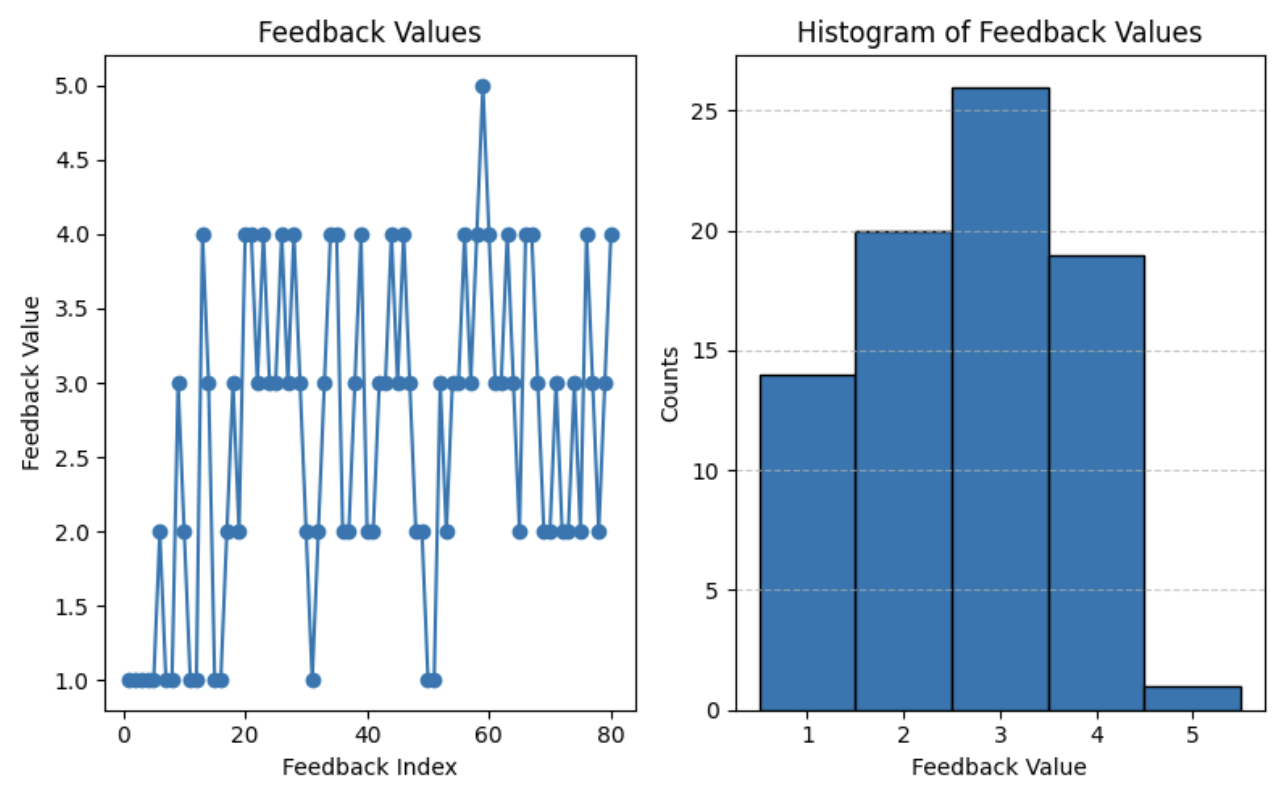
\includegraphics[width=14cm]{results.png}
    \centering
    \label{111}
\end{figure}
\\
As depicted in Figure \ref{111}, it can be observed that user feedback slightly improved over time, indicating that the movements appeared more pleasant to users as training progressed.
Another measurable aspect was the average feedback score provided by users, which was also at 3. From the histogram in Figure 1, it is evident that there were very few instances where a rating of 5 was given.
Additionally, it is noticeable that users most frequently gave a rating of 3, suggesting that the movements were moderately good.
\\
Overall, while it was difficult to quantify improvements in movement quality, the feedback trend and average scores suggest a modest level of effectiveness in the implemented method.

\subsection{Materials}

\begin{itemize}
    \item \href{https://scm.cms.hu-berlin.de/adapt/teaching/ws23-smlr/g4-user_feedback.git}{https://scm.cms.hu-berlin.de/adapt/teaching/ws23-smlr/g4-user\_feedback.git}
    \item examples from the dmpbbo git~\cite{stulp2019dmpbbo}
    \item QiBullet~\cite{QiBullet}
\end{itemize}




\section{Discussion/Conclusion}

Training robots with user feedback is a crucial aspect of robotics research and development. The integration of user feedback enables robots to adapt and improve their behavior based on real-world interactions, enhancing their usability and applicability in various contexts. This approach aligns with the principles of human-robot interaction (HRI), where seamless communication and collaboration between humans and robots are essential for effective task completion.
\\
The implementation of a tool capable of optimizing simulated movements with user feedback marks a significant step towards enabling intuitive robot skill learning. However, our endeavor encountered several challenges and limitations, prompting considerations for future research and development.
\\
One primary challenge was optimizing movements effectively, given the simplicity of the tasks implemented. The inherent difficulty in evaluating and quantifying improvements in basic movements made it challenging to gauge the effectiveness of the optimization process accurately. Furthermore, users struggled to make direct comparisons between iterations of movements due to subtle improvements over time. As a result, assessing the efficacy of the learning algorithm became a non-trivial task.
\\
Despite these challenges, the iterative nature of the feedback loop demonstrated promising potential for enhancing movement quality over time. The slight improvement observed in user feedback over successive iterations suggests that the learning algorithm effectively incorporated user input to refine movements incrementally. This iterative improvement highlights the adaptability and flexibility of the optimization approach, which can iteratively adjust movement parameters based solely on user feedback.
\\
However, the limitations of our study underscore the need for further exploration and refinement. One avenue for future research involves expanding the scope of movements to include more complex tasks. By introducing a wider variety of movements, each with its unique challenges, we can better assess the algorithm's performance across different contexts. Additionally, incorporating a slider interface, as suggested, could facilitate the execution of more diverse movements and provide users with greater control and granularity in providing feedback.
\\
In conclusion, while our approach faced challenges in optimizing simulated movements with user feedback, it highlights the potential of this approach for intuitive robot skill learning. By addressing the identified limitations and exploring avenues for improvement, future research can continue to advance the field, ultimately enabling robots to learn and adapt to tasks more effectively in real-world environments.

\subsection*{Author contributions}

Simon Maximilian Friedo implemented most of the code for training the robot using the dmpbbo package~\cite{stulp2019dmpbbo}
and for sending the trajectories to the simulation using QiBullet~\cite{QiBullet}.
He also wrote multiple parts of this seminar paper. \newline \newline
Marvey Bano worked with the initial simulation of Pepper's movement and wrote the simulation subsection of this seminar paper.
\newline \newline
Sedra Abou Ghaloun implemented the simulation code for both simple and complex movements. Additionally, she integrated sliders into the graphical user interface (GUI) to facilitate the export of initial trajectories. Furthermore, she was responsible for generating the results, evaluating the data from our experiments, and writing the results and evaluation sections of this seminar paper.
\newline

\bibliographystyle{alpha}
\bibliography{sample}

\end{document}
